\documentclass[a4paper]{article}
\usepackage{praktikum}
\begin{document}
	
%%
%% Bitte das Deckblatt nicht verändern


\thispagestyle{empty}
\begin{center}

    {\large {\bf   BAI3-GKA WiSe2§ \\ Graphentheoretische Konzepte und Algorithmen \\[5mm]} }
    
{\huge Praktikumsaufgabe-Template  \\[5mm] Deckblatt}\\

\end{center}

				\begin{tabular}[t]{|r|l|}
				 \hline
%%%%				
%%%% Bitte  Ihren Namen und  Ihr Team und die Gruppe angeben
				GKA-Gruppe&                 \raisebox{-3mm}{\rule[8mm]{100mm}{0mm} }\\ \hline    
				Team &                                                        \\ \hline			
				& \textit{Iryna Trygub }               \\ \hline    
				& \textit{Ansgar Deuschel }               \\ \hline			
				& \textit{Kristoffer Schaaf }             \\ \hline  			
				\multicolumn{2}{c}{}\\  			
				\multicolumn{2}{l}{Bearbeitete Themen in Stichpunkten:}\\			
				\multicolumn{2}{c}{}\\  \hline
				Iryna Trygub &              \\ \hline    
				Ansgar Deuschel &                \\ \hline			
				Kristoffer Schaaf & Ops            \\ \hline 		
				\multicolumn{2}{c}{}\\  			
				\multicolumn{2}{l}{Geschätzte Arbeitszeiten in Stunden:}\\			
				\multicolumn{2}{c}{}\\  \hline
				Iryna Trygub &               \\ \hline    
				Ansgar Deuschel &                \\ \hline			
				Kristoffer Schaaf &               \\ \hline 			
				\end{tabular}
~\\[4mm]
		
		
\vfill


\newpage

\tableofcontents

\newpage

\section{Einleitung}

\subsection{Dijkstra Algorithmus in Worten}

Wie genau funktioniert der Dijkstra Algorithmus und wo wird er angewendet?
Nehmen wir an Kreuzungen und Kreisverkehre seien Knoten und die Straßen, die diese verbinden die Kanten. Dann lässt sich bis auf Ausnahmen jedes Straßennetz durch einen Graphen darstellen. Um zu berechnen, wie Mensch am schnellsten von einem beliebigen Kreisverkehr zu einer beliebigen Kreuzung kommen kann, wird nun zum Beispiel der Dijkstra Algorithmus verwendet.

\begin{enumerate}
    \item Finden des Startknotens im Graphen.
    \item Dann die Distanz zu allen adjazenten Knoten berechnen und diese zusammen mit der Distanz zum Startknoten und den Knoten auf dem Weg dorthin in einer Open List speichern. 
    \item Den Ausgangsknoten auf eine Closed List verschieben, da alle inzidenten Kanten bearbeitet wurden.
    
    \item Nun den Knoten mit kürzester Distanz zum Startknoten in der Open List suchen und Schritt 2 von diesem Knoten aus wiederholen
    \begin{enumerate}
        \item Wenn ein Knoten, welcher bereits in der Open List gespeichert ist, erneut besucht wird, dann wird verglichen ob die neue Distanz kürzer ist. Wenn ja, wird der Knoten inklusive der Distanz zum Startknoten und den Knoten auf dem Weg dorthin aktualisiert. Wenn die Distanz länger ist, wird der Weg verworfen.
        \item Wenn alle inzidenten Kanten eines Knotens bearbeitet wurden, wird dieser Knoten in die Closed List verschoben.
    \end{enumerate}

    \item Der Algorithmus ist beendet, wenn entweder
    \begin{enumerate}
        \item alle Knoten des Graphen besucht wurden oder
        \item die Distanz vom Start- zum Zielknoten, die bisher kleinste gefundene Distanz ist.
    \end{enumerate}
\end{enumerate}

\subsection{Wählen des Grundansatzes}

Zur objektorientierten Abstrahierung eines Graphen gibt es zwei verschiedene Ansätze. Der erste Ansatz wäre, dass es einen Typen \textit{Kante} gibt, in welchem die vor- und nachfolgenden Knoten und die Länge der jeweiligen Kante gespeichert werden.\\
Diese Kanten würde dann den Graphen bilden und diesen in Form eines Sets darstellen:\\$Set <Kante> graph = new\ HashSet<>()$.\\\\
Der zweite Ansatz wäre die Kante als solches zu abstrahieren und nicht als eigenen Typen zu implementieren. Es gäbe dann nur den Typen Knoten, welcher alle benachbarten Knoten mit zugehöriger Distanz enthält.\\
Auch diese Knoten können nun in einem Set gespeichert werden:\\
$Set<Knoten> graph = new\ HashSet<>()$.\\\\
Die zu verwendende Java Bibliothek Graphstream enthält einen Typen Multigraph, welcher den ersten Ansatz implementiert.\\
Eine Beispiel Implementierung des zweiten Ansatzes ist im folgenden Blog Eintrag\footnote{\url{https://www.baeldung.com/java-dijkstra}} implementiert.



\subsection{Aufbau des Graphen}

Um den Dijkstra Algorithmus innerhalb eines Graphen anwenden zu können, muss zuerst ein Graph aufgebaut werden.
Wie im vorherigen Kapitel beschrieben, genügt es einen Multigraphen zu definieren und diesem Kanten hinzuzufügen.
Sowohl die Kanten als auch die Knoten müssen einen eindeutigen, im Graphen nur einmal vorkommenden Namen haben.\\\\
Bedingungen, welche für den Graphen gelten:
\begin{itemize}
    \item Der Graph muss vollständig gewichtet sein und ausschließlich positive Kantengewichte haben.
    \item Der Graph kann unendlich viele Knoten besitzen.
    \item Der Graph kann gerichtet, ungerichtet oder gemischt sein.
    \item Der Graph darf Schleifen, aber keine nicht inversen Multikanten besitzen.
\end{itemize}

\subsection{Open und Closed List}

Knoten in der Closed List dienen der Kontrolle ob alle Kanten eines neu gefundenen Knoten bereits besucht wurden. Wird ein neuer Knoten gefunden, welcher noch nicht in der Open List enthalten ist, muss nun kontrolliert werden ob dieser bereits vollständig abgearbeitet ist, d.h. ob alle inzidenten Kanten bereits geprüft wurden.\\
Es reicht ein einfaches Set, welches die bereits besuchten Knoten enthält: $Set<Knoten>\ closedList$. Durch die Verwendung eines Sets wird außerdem das mehrfache Hinzufügen eines Knotens verhindert.\\\\
In der Open List wird der derzeitige Fortschritt festgehalten. Die verschiedenen Elemente können als Tabelleneintrag gespeichert werden. Eine Zeile dieser als Tabelle dargestellten Open List könnte folgendermaßen definiert werden:

\begin{table}[htbp]
    \centering
    \begin{tabular}{||l|l|l|l||}
    \hhline{|t:====:t|}
    \textbf{Beschreibung}   & Knoten  & Länge zum Startknoten & Knoten auf dem Weg    \\ \hhline{|----|}
    \textbf{Typ}            & Node    & Integer               & $List<Knoten>$        \\ \hhline{|----|}
    \textbf{Beispiel}       & ''D''   & 44                    & \{\{''A'', ... \},\{''C'', ... \}\}           \\ \hhline{|b:====:b|}
    \end{tabular}
    \caption{Open List}
\end{table}

\subsubsection{Open List als Set}

Auch wenn es dem Namen widerspricht, kann die Open List als Set implementiert werden. Wenn ein Knoten hinzugefügt wird, muss erst geschaut werden ob dieser schon vorhanden ist. Zum Vereinfachen dieser Suche wird eine Map genutzt: $Map<Knoten,\ Weg>\ openList$, wobei der Weg die Distanz zum Startknoten und die Knoten auf diesem Weg enthält. Wenn der Knoten nicht vorhanden ist, wird der Map ein neues Element hinzugefügt, welches als Key den neuen Knoten und als Value dessen Distanz zum Startknoten und den Knoten auf diesem Weg enthält.\\
Nach jeder Iteration muss der Knoten aus der Open List mit dem kürzestem Weg zum Startknoten bestimmt werden. Mit dieser Struktur ist dieser Prozess mit viel Rechenaufwand verbunden.

\subsubsection{Open List als Priority Queue} \label{priorityQueueSection}

Java bietet einen Typen Priority Queue an. Diesem kann eine Comparator übergeben werden, welcher die in der Queue enthaltenden Elemente effizient nach bestimmten Attributen sortiert.\\
So können zum Beispiel verschiedene Listen mit Knoten beim Einfügen von Elementen direkt nach der in den Knoten enthaltenden Länge zum Startpunkt sortiert werden.\\
Ein großer Vorteil, den diese Implementierung mit sich bringt ist, dass durch die Funktion\\$PriorityQueue.peak()$ effizient der Knoten für die Wiederholung des Algorithmus bestimmt werden kann.\\
Der Typ Knoten muss des weiteren nur noch die adjazenten Knoten mit der Distanz enthalten.\\

\section{Dokumentation der Implementierung}

\subsection{IO}

\subsubsection{Dateiformat}
\label{Dateiformat}
Gelesen und geschrieben wird in eine *.grph Datei, deren Aufbau folgendermaßen strukturiert ist:
\begin{enumerate}
 	\item Kopfzeile beginnt mit '\#' worauf das Schlüsselwort  \verb"undirected", bzw. \verb"directed", ein Doppelpunkt und der Name des Graphen folgt. Wie jede Zeile wird die Kopfzeile durch ein Semikolon abgeschlossen:\\
		\verb|#<(un)directed>:name;|
	\item Alle folgenden Zeilen beinhalten entweder einen Knoten mit optionalem Attribut \verb|(":" als Präfix):| \\
		\verb|<Knotenname>(:Attribut)?;|
	\item oder zwei Knoten mit jeweils optionalen Attributen, sowie darauf folgend optional explizitem Kantennamen (umklammert) und/oder Kantengewicht \verb|("::" als Präfix):|\\
		\verb|<Knotenname1>(:Attribut)?-<Knotenname2>(:Attribut)?((<Kantenname))?(::<Kantengewicht>)?|
    \item Graphen, die sowohl ungewichtete, als auch gewichtete Kanten besitzen, werden nicht akzeptiert, da diese hier keine algorithmische Anwendung finden, ohne Knotengewichte zu erfinden.
\end{enumerate}

\subsubsection{Lesen der Graphdatei}
Gelesen wird die Graphdatei in der Klasse \verb|GraphFileReader| mit einem nach ISO-8859-1 encodierten \verb|InputStreamReader|. Hier kann eine \verb|IOException| geworfen werden.\\
Nachdem die Zeilen eingelesen wurden, wird jede Zeile mit Regex auf Korrektheit, wie in \ref{Dateiformat} beschrieben, geprüft. Diese Prüfung ist in der Klasse Verifier implementiert.\\ \\
Die Funktionsweise der Regexprüfung baut auf dem Erkennen und Löschen der Zeilenbestandteile (Quell-/Ziel-)Knoten, Knotenattribut, Kantenname und Kantengewicht auf. Wenn alle Bestandteile aus der Zeile gelöscht sind, darf nur noch das Semikolon übrigbleiben. Dieses vorgehen verhindert, dass Attribute wie Kantengewicht oder Kantenname doppelt oder in einer
Zeile mit nur einem Knoten vorkommen, und dass pro Zeile nur maximal zwei Knoten (als Kante) vorkommen dürfen.\\ \\
Ist die Prüfung erfolgreich, kann einem neuen Graphenobjekt der entsprechenden Bibliothek von graphstream.org die in der Zeile genannten Eigenschaften hinzugefügt werden. Dies übernimmt die Funktion \verb|addProperties(Graph, Zeile)| in der \verb|GraphFileReader-Klasse|.\\
Ähnlich wie bei der Regexprüfung werden hier zur Vereinfachung des Patternmatchings identifizierte Attribute aus der zu lesenden Zeile gelöscht, nachdem sie in einer lokalen Variable gespeichert wurden. Und da die Korrektheit der Zeile bereits bewiesen ist, kann man durch Teilung an definierten Zeichen weitere semantischen Bestandteile der Zeile erhalten, nachdem die hintenstehenden Attribute Kantenname und Kantengewicht entfernt wurden. Teilt man den übriggebliebenen String am Zeichen "-", erhält man beide Knoten getrennt und teilt man diese jeweils am Zeichen \verb|":"|, erhält man deren Attribut.\\
Wenn alle in der Zeile angegebenen Attribute in lokalen Variablen gespeichert sind, kann man auf deren Grundlage die Objekte \verb|"Node"| und \verb|"Edge"| dem übergebenen Graphobjekt hinzufügen. Zur verbesserten Darstellung werden die Knoten- und Kantennamen als ui.label jeweils hinzugefügt.\\ \\
Sind alle Zeilen abgearbeitet, wird geprüft ob der Graph ungerichtete und gerichtete Kanten gleichzeitig enthält und in diesem Fall aussortiert. Zudem wird für eine potentielle spätere Verwendung im Graph die Information aufgenommen, ob dieser gerichtet ist, oder nicht. Anschließend erhält man das fertige Graphobjekt von der Methode \verb|getGraphFromFile| zurück.\\

\subsubsection{Schreiben der Graphdatei}
Geschrieben wird das Graphobjekt der Bibliothek von graphstream.org im gleichen Format wie in \ref{Dateiformat} beschrieben.\\
Die Methode \verb|writeFile(Graph, Filename)| iteriert hier erst über die Kantenobjekte und konkatiniert deren Bestandteile Quell-/Zielknoten, Kantengewicht und Kantenname zu einem Outputstring, die mit Semikolon und Zeilenumbruch nach korrekter Syntax abgeschlossen wird.\\
Anschließend wird zur Berücksichtigung von Knoten ohne Nachbarn nochmals über die Knoten iteriert, um diese zu identifizieren und ggf. dem Outputstring hinzuzufügen. Dieses doppelte Iterieren reduziert die Verschachtelung von Logik im Vergleich zum einfachen Iterieren über alle Knoten, von denen die bereits abgearbeiteten gebuffert werden müssten, um mehrfache Einträge einer gleichen
Kante zu erkennen.\\
		

\subsection{Einführung neuer Typen}

Wie bereits in \ref{priorityQueueSection} beschrieben, ist die Implementierung der Open List als PriorityQueue am sinnvollsten.\\\\
Zur effizienteren Sortierung wird einer neuer Typ \textit{PriorityQueueItem} eingeführt.\\

\begin{lstlisting}[language = java, frame = trBL]
@Data
@NoArgsContructor
public class PriorityQueueItem {

    /* Um das Item bei falscher Initialisierung nicht auf die
    erste Position in der PriorityQueue zu schieben, wird es mit einer
    maximalen Distanz initialisiert.*/
    private int distance = Integer.MAX_VALUE; 

    /*Die Reihenfolge dieser Knoten muss beibehalten werden,
    da ansonsten der kuerzeste Weg nachtraeglich nicht zurueckgegeben
    werden kann*/
    private List<Node> nodes = new LinkedList<>(); //Node -> Knoten
}
\end{lstlisting}

\newpage

\subsection{Ablauf des Algorithmus mit einer Priority Queue}

\begin{enumerate}
    \item Ein leeres $Set<Node>\ closedList$ und eine leere $PriorityQueue<PriorityQueueItem> priorityQueue$ werden initialisiert.
    \item Für den Startknoten wird ein \textit{PriorityQueueItem} initialisiert und der \textit{priorityQueue} hinzugefügt. Dieses hat eine \textit{distance} von 0 und der \textit{nodes} Liste wird der Startknoten hinzugefügt.
    \item Jeder adjazente Knoten des Ausgangsknotens wird betrachtet:
    \begin{enumerate}
        \item Ist der Knoten bereits in der closedList: Knoten muss nicht weiter beachtet werden.
        \item Für jeden weiteren wird ein neues \textit{PriorityQueueItem} initialisiert. Die \textit{distance} ist die Distanz zwischen dem Ausgangsknoten und dessen adjazentem Knoten. Die \textit{nodes} Liste enthält den neuen Knoten.\\Diese neuen \textit{PriorityQueueItems} werden nun jeweils mit dem bereits bestehendem \textit{PriorityQueueItem} des Ausgangsknotens ergänzt. Hierbei werden die Distanzen aufsummiert und die Listen konkateniert (Reihenfolge beachten).
    \end{enumerate}
    \item Die neu entstandenen \textit{PriorityQueueItems} ersetzen nun das \textit{PriorityQueueItem} des Ausgangsknotens in der \textit{PriorityQueue} unter folgender Bedingung:
    \begin{enumerate}
         \item Ist der letzte Knoten aus der \textit{nodes} Liste einer dieser \textit{PriorityQueueItems} bereits das letzte Element einer \textit{nodes} Liste eines \textit{PriorityQueueItems} in der \textit{PriorityQueue} muss verglichen werden, welche \textit{distance} der \textit{PriorityQueueItems} kleiner ist und nur dieses \textit{PriorityQueueItem} wird behalten.
    \end{enumerate}
    \item Da alle Kanten des Ausgangsknotens jetzt untersucht wurden, wird dieser der \textit{closedList} hinzugefügt.
    \item Das oberste Element der \textit{PriorityQueue} wird bestimmt. Das letzte Element aus dessen \textit{nodes} Liste wird zum neuen Ausgangsknoten und Schritt 3 wird wiederholt.
    \item Der Algorithmus ist beendet, wenn entweder
    \begin{enumerate}
        \item alle Knoten des Graphen besucht wurden oder
        \item der Zielknoten das letzte Element der \textit{nodes} Liste eines bereits in der \textit{PriorityQueue} enthaltendem \textit{PriorityQueueItem} und die \textit{distance} die bisher kleinste gefundene Distanz ist.
    \end{enumerate}
\end{enumerate}

\begin{figure}[htbp]
	\centering
		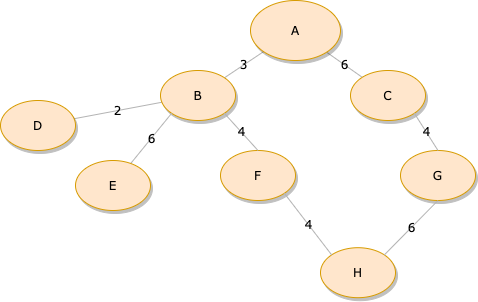
\includegraphics[width=0.60\textwidth]{Figs/Beispielgraph_2.png}		
	\caption{Gewichteter, ungerichteter Graph}
	\label{fig:beispielgraph_2}
\end{figure}

\subsubsection{Beispiel}

Sei der Knoten ''A'' auf folgendem Graphen~\ref{fig:beispielgraph_2} ein Startknoten.
Nach zwei Iterationen sieht der Inhalt der PriorityQueue wie folgt aus:\\

\begin{lstlisting}[language = java, frame = trBL]
priorityQueue = {
    {5, {A, B, D}},
    {6, {A, C}},
    {7, {A, B, F}},
    {9, {A, B, E}}
};

closedList = { };
\end{lstlisting}

\subsection{Rekursive Implementierung des Dijkstra-Algorithmus}
Neben dem iterativen Ansatz haben wir eine rekursive Methode zur Implementierung des Dijkstra-Algorithmus umgesetzt. Ähnlich wie beim vorherigen Verfahren wurde eine Priority Queue eingesetzt, um die Knoten effizient nach ihrer Entfernung zum Startknoten zu sortieren und auszuwählen. Bereits besuchte Knoten werden, wie im vorherigen Verfahren, in einem Set gespeichert. 
In der Hauptfunktion \textit{calculateFastestPathRecurs} erfolgt die Initialisierung der \textit{PriorityQueue} sowie der \textit{closedList}. Daraufhin wird ein erstes \textit{PriorityQueueItem} basierend auf dem Startknoten definiert. Die \textit{finalPathsQueue} hält die Endergebnisse der Rekursion fest, um einen korrekten Rückgabewert sicherzustellen.
Die Funktion \textit{recursStep} stellt den rekursiven Schritt dar, der die Kernlogik des Algorithmus beinhaltet. In jedem Rekursionsschritt wird das erste Element der \textit{PriorityQueue} verarbeitet, ähnlich wie im iterativen Ansatz. Das Abbruchkriterium der Rekursion ist erreicht, wenn der Knoten aus dem aktuellen \textit{PriorityQueueItem} der Zielknoten ist und alle Knoten besucht wurden. Dann wird dieser in die \textit{finalPathsQueue} aufgenommen. Diese enthält alle Pfade, die am Zielknoten enden. Beim Verlassen der Rekursion wird die \textit{finalPathsQueue} zurückgegeben und im Methodenaufruf von \textit{calculateFastestPathRecurs} wird das erste Element dieser Queue entnommen, welches den optimalen Pfad repräsentiert.
Sollte der Knoten aus dem aktuellen \textit{PriorityQueueItem} nicht der Zielknoten sein, so werden die adjazenten Knoten überprüft. Jeder dieser Knoten wird daraufhin kontrolliert, ob er bereits in einem der potenziellen Pfade in der \textit{PriorityQueue} enthalten ist. Wenn dies der Fall ist und der neu berechnete Pfad ist kürzer, wird auf Basis des gefundenen Pfades ein neues \textit{PriorityQueueItem} erstellt und die Distanz entsprechend aktualisiert. Sollte der adjazente Knoten noch nicht in den vorhandenen Pfaden sein, wird auch ein neues \textit{PriorityQueueItem} mit diesem Knoten angelegt.
Nachdem alle adjazenten Knoten verarbeitet wurden, wird das aktuelle \textit{PriorityQueueItem} aus der \textit{PriorityQueue} entfernt. Anschließend wird ein neuer rekursiver Schritt für die aktualisierte \textit{PriorityQueue} aufgerufen.

\section{Tests}

Um das Program zu überprüfen, ist es notwendig aussagekräftige Tests zu implementieren. Dazu haben wir das JUnit Jupiter Testframework verwendet, ein Java-Test-Framework, welches die Erstellung und Ausführung von Unit-Tests automatisieren und vereinfachen soll.\\

Unsere Tests decken folgende Fälle ab:

\begin{enumerate}
    \item Testen von gerichteten Graphen
    \item Was passiert, wenn der Startknoten auch der Endknoten ist.
    \item Funktioniert die Anwendung bei einem Graph mit einer Schleife.
    \item Was ist, wenn der gesamte Pfad den Wert 0 hat.
    \item Wird eine NodeNotFoundException geworfen, wenn der Start- oder Endknoten nicht im Graphen enthalten sind.
    \item Wird eine MultiEdgeWithSameDirectionException geworfen, wenn eine entsprechende nicht inverse Multikante gefunden wurde.
    \item Wird eine UnoperableGraphException vom Algorithmus geworfen, wenn der Graph ungewichtet ist.
    \item Wird eine UnoperableGraphException von der GraphFileReader-Klasse geworfen, wenn der Graph gemischt ungewichtet und gewichtet ist.
\end{enumerate}


\end{document}